\section{Statistical analysis}
\label{sec:statistical_analysis}

\todo[inline]{Fit, limits, treatment of systematics in fit}

Directly fit MVA score.

\Cref{sec:statistical_methods} introduced the methods that are used
for the statistical analysis.

\todo[inline]{Maybe say something about blinding?}

\todo[inline]{Chapter with validation plots before this one?}

\subsection{Re-binning algorithm}
\label{sec:binning_alg}

\todo[inline]{Move to signal / background model?}

The signal sensitivity of a binned maximum likelihood fit of
MVA scores depends strongly on the choice of binning used for the
discriminant. The purity of signal increases with increasing MVA
score, with most signal (background) being concentrated at the highest
(lowest) MVA scores. For optimal expected signal sensitivity, the
binning has to be chosen such that regions in MVA score with low
signal-to-background ratio are separated from regions with high
signal-to-background ratio.

In this analysis an iterative re-binning algorithm is used to provide
the binning of the discriminants for the likelihood fits. The aim of
the algorithm is to provide good expected signal sensitivity while
ensuring that the background model obeys predefined constraints on the
statistical uncertainty and expected number of events in each bin. The
constraints are intended to stabilise the likelihood fits and ensure
reasonable validity of the asymptotic approximations used for the
sampling distributions of test statistics used in the statistical
analysis. The algorithm was previously used
in~\cite{HIGG-2016-16-witherratum} and is continued to be used in the
\hadhad channel of this search. A different algorithm, while
conceptually similar, is used in the \lephad channel and is
detailed~\cite{ATLAS-CONF-2021-030}.

The re-binning algorithm is provided with MVA score histograms with
fine, equidistant binning ($N_\text{bins} = 1000$) for the signal and
total background expectation. It proceeds by iteratively merging bins,
starting from the most-signal like MVA score bins, until the bin
fulfills a set of requirements:
\begin{enumerate}

\item The relative statistical uncertainty of the background in the
  bin must be smaller
  than~\mbox{$\SI{50}{\percent} \cdot f_\text{s} + \SI{1}{\percent}$},
  where $f_\text{s}$ is the fraction of signal events entering the bin
  relative to the expected number of signal events in the signal
  region. This requirement limits the statistical uncertainty on the
  background in the most signal-like bins after re-binning to be in
  the range of \SIrange{10}{20}{\percent}.

\item The expected number of background events in the bin must be
  larger than 5.

\end{enumerate}
When a bin fulfilling all requirements is found, the process is
repeated starting from the next un-merged bin. The algorithm
terminates with a final bin at low MVA score. If the final bin does
not fulfil the criteria, it is merged with the preceeding (already
merged) bin.

% The algorithm provides a binning that improves the analysis
% sensitivity while fulfilling criteria on the background model:
% I.e. that it has reasonable statistical precision, and that one
% expects at least 5 events so that asymptotic approximations of the
% test statistics can be used.

% Motivation of terms:
% 1\% have some bins in background dominated region
% signal fraction weighted 50\% to have relatively fine bins in the most signal-like regions

The size of bins resulting from the re-binning procedure can vary by
multiple orders of magnitude. For better visualisation of the bin
contents, the MVA scores are displayed as equidistant bins.

\todo[inline]{Visualise the rebinning somehow?}


\subsection{The signal and background model}

\todo[inline]{Signal is ggF + VBF}
\todo[inline]{Reminder of freely floating backgrounds}
\todo[inline]{Emphasise that there are really many models for each MVA score that is fit.}
\todo[inline]{Models developed in a blind analysis (blind -> high MVA score region blinded)}

\subsubsection{Re-binning algorithm}
\subsubsection{Interpolation and symmetrisation}
\subsubsection{Smoothing and pruning}
\subsubsection{Nuisance parameter correlation scheme}
\subsubsection{Model validation}

\subsection{Results of the search for non-resonant production of SM $HH$}


\begin{figure}[htbp]
  \centering

  \begin{subfigure}{0.495\textwidth}
    \centering

    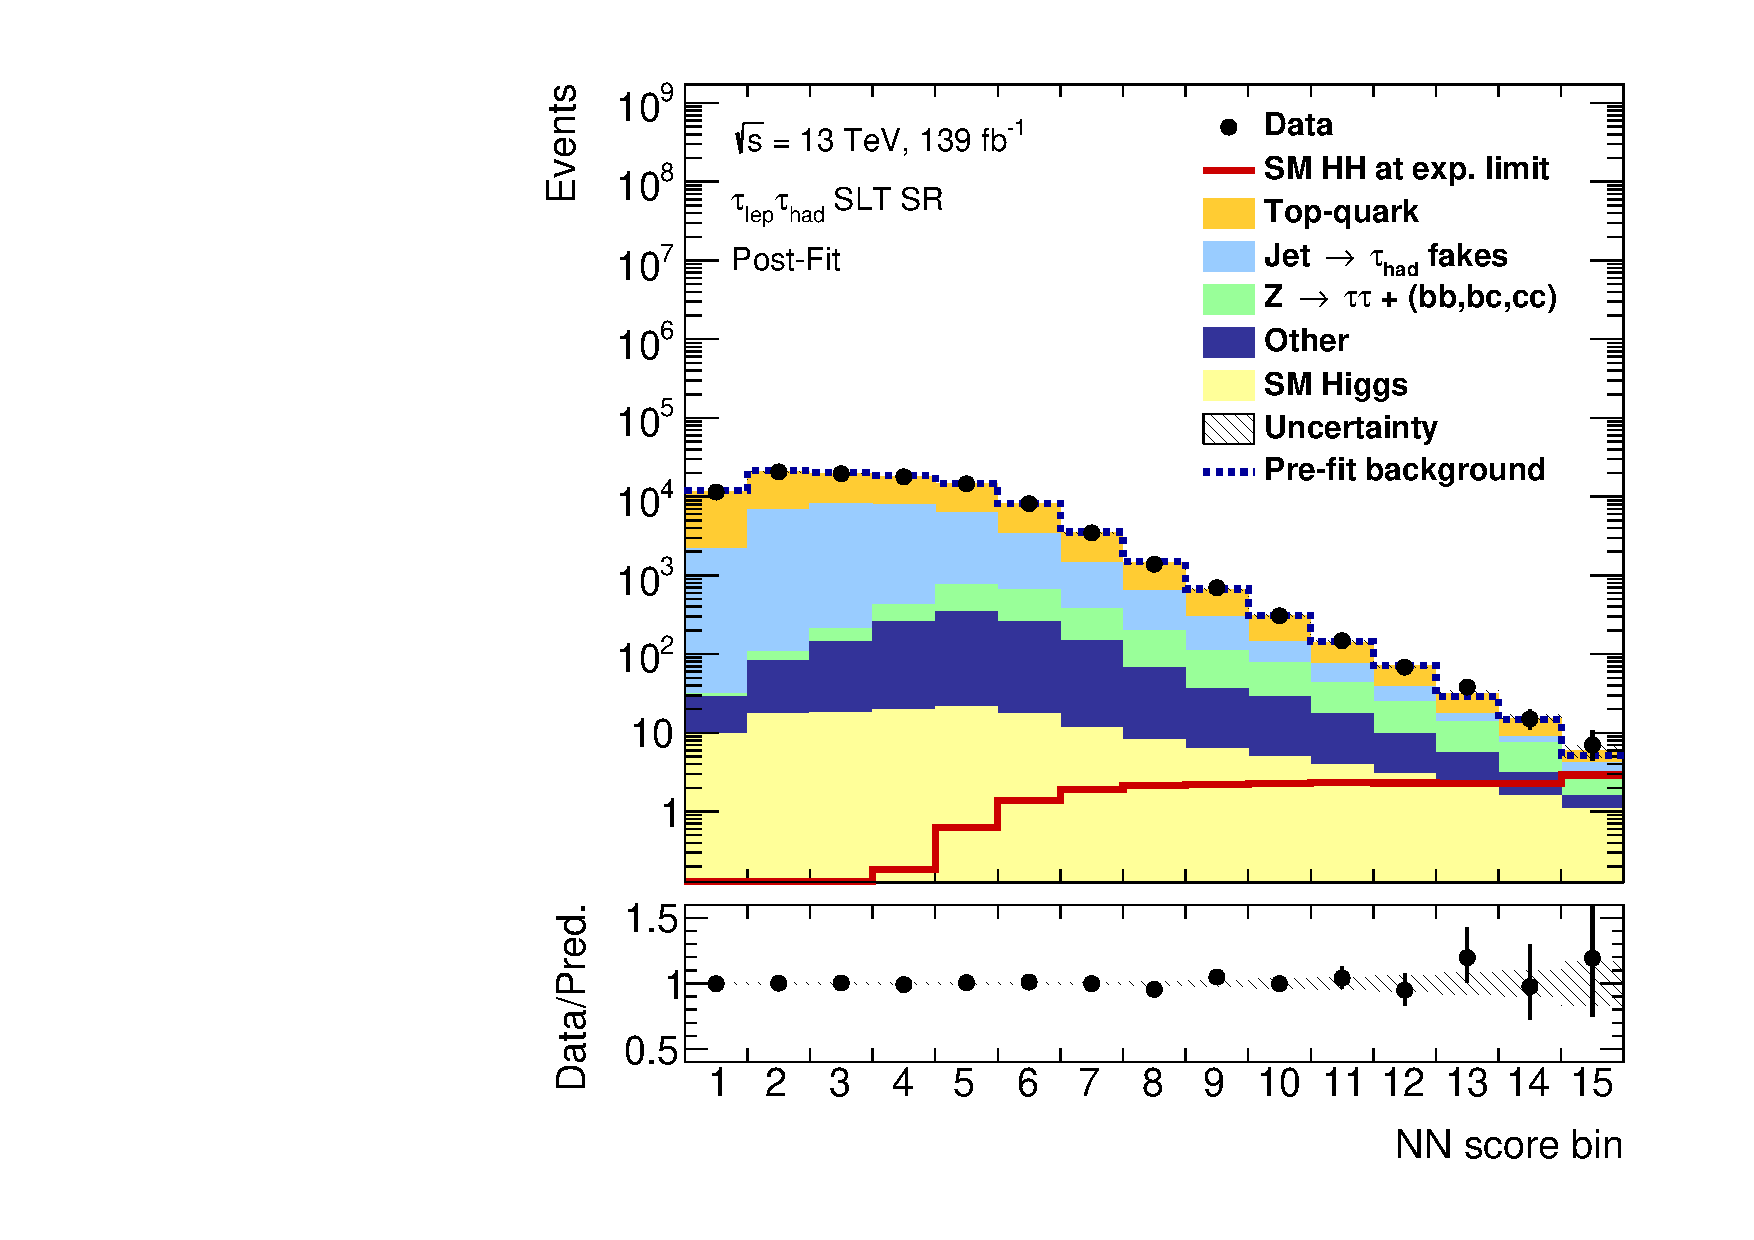
\includegraphics[width=\textwidth]{results_nonres/postfit/Region_BMin0_incJet1_distNN_J2_DSM_T2_SpcTauLH_Y2015_LTT0_L1_GlobalFit_conditionnal_mu0log}

    \subcaption{\lephad SLT channel}
  \end{subfigure}\hfill%
  \begin{subfigure}{0.495\textwidth}
    \centering

    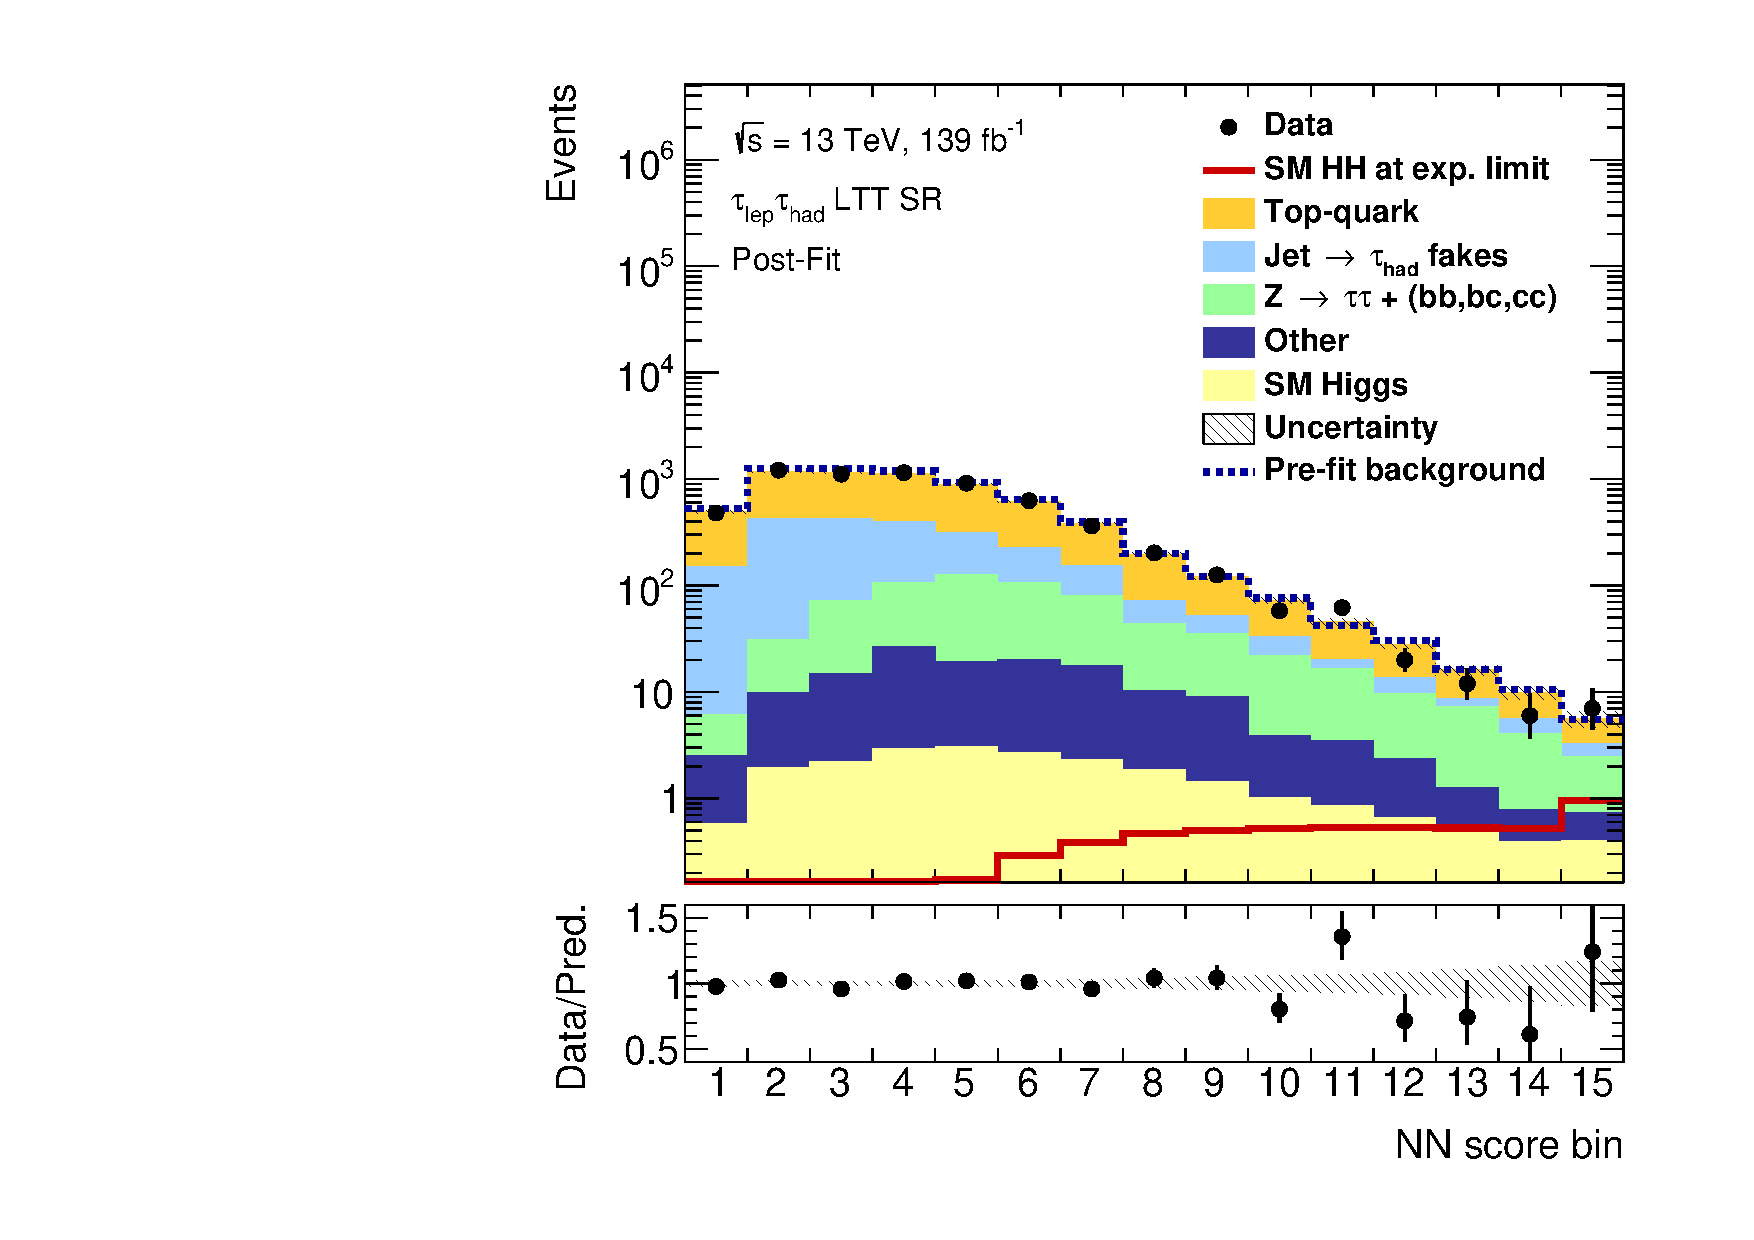
\includegraphics[width=\textwidth]{results_nonres/postfit/Region_BMin0_incJet1_distNN_J2_DSM_T2_SpcTauLH_Y2015_LTT1_L1_GlobalFit_conditionnal_mu0log}

    \subcaption{\lephad LTT channel}
  \end{subfigure}

  \vspace{0.5em}

  \begin{subfigure}{0.495\textwidth}
    \centering

    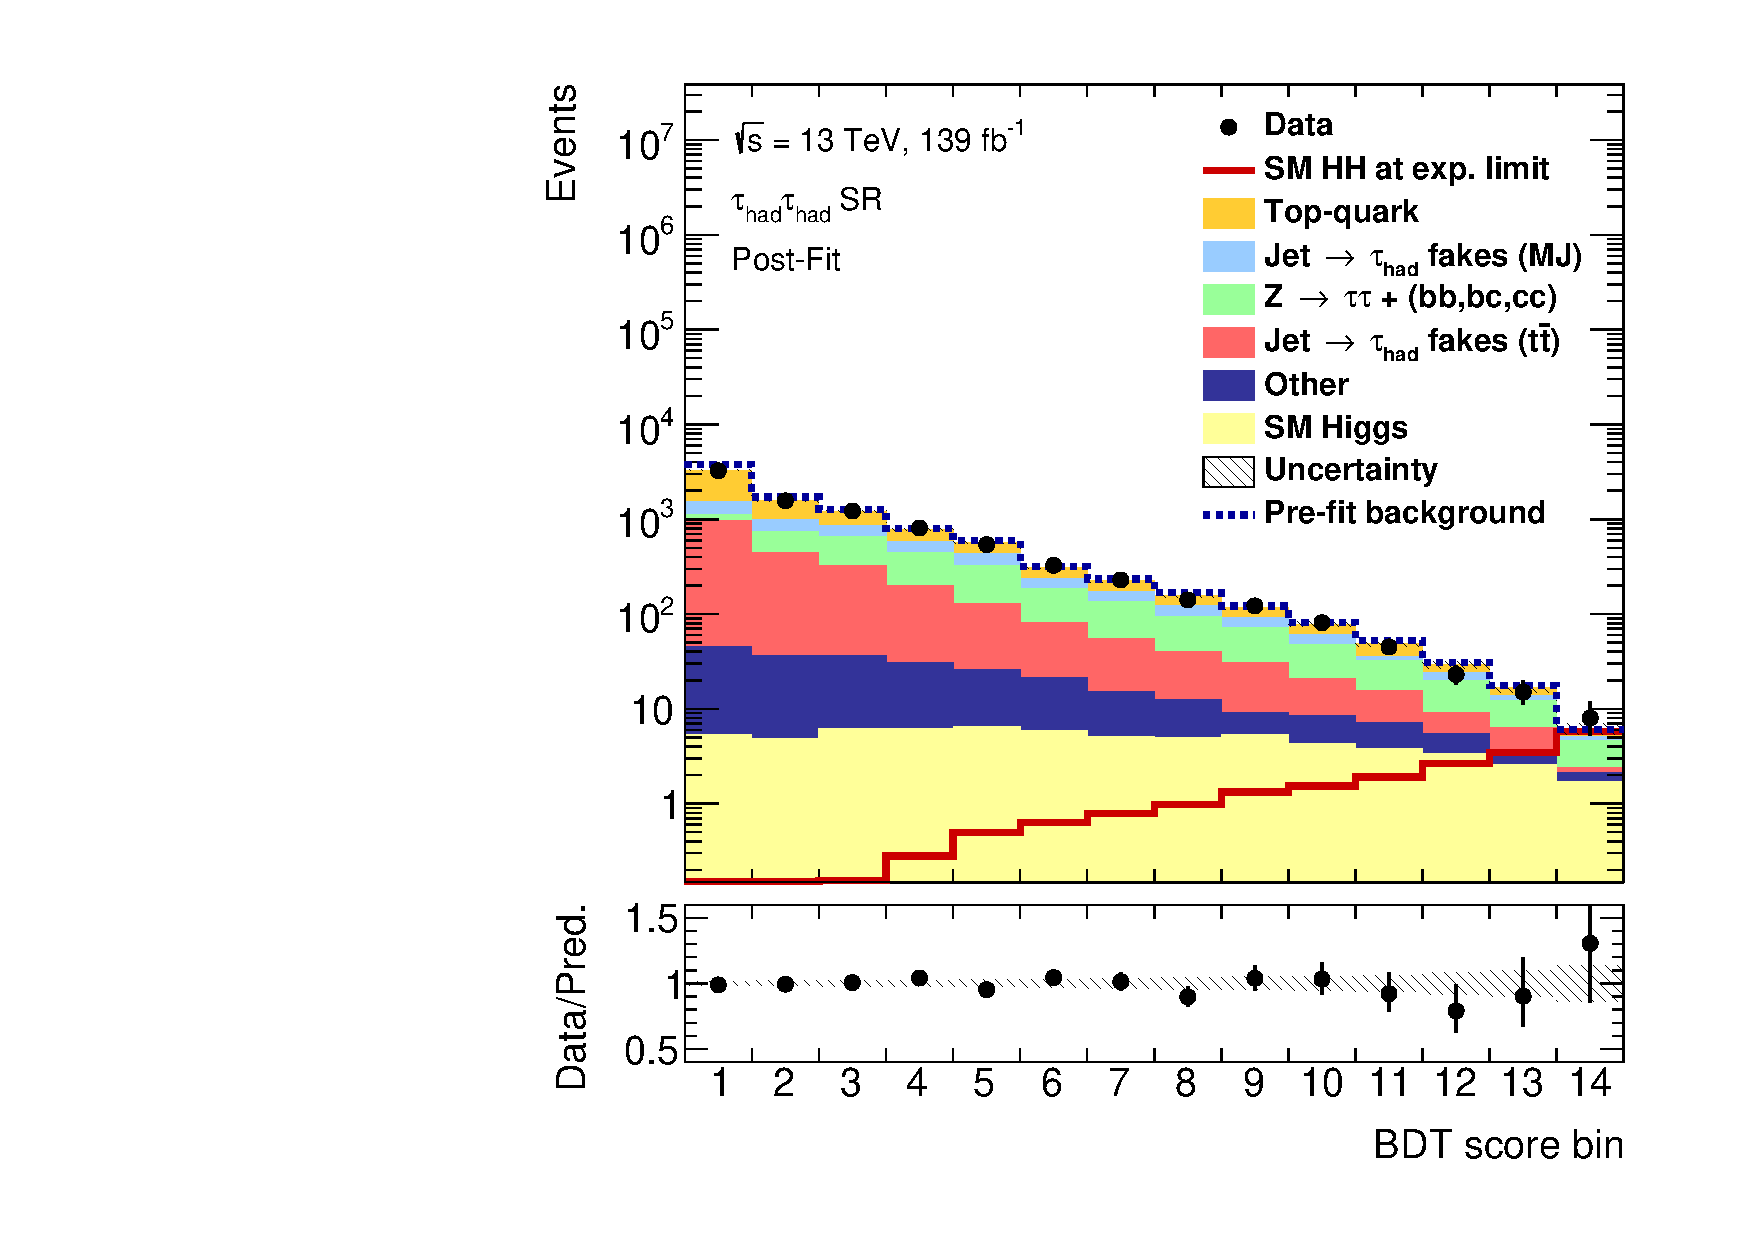
\includegraphics[width=\textwidth]{results_nonres/postfit/Region_BMin0_incJet1_distSMBDT_J2_Y2015_DLLOS_T2_SpcTauHH_L0_GlobalFit_conditionnal_mu0log}

    \subcaption{\hadhad channel}
  \end{subfigure}

  \caption{Distribution of the MVA discriminants used to extract the
    non-resonant SM \HH signal in the \lephad SLT (a), \lephad LTT
    (b), and \hadhad (c) channel after the background-only fit of all
    signal and control regions. The signal overlay is scaled to the
    expected upper limit on the signal strength of $3.9$ from the
    combination of all channels.}
\end{figure}



\begin{figure}[htbp]
  \centering

  \begin{subfigure}{0.46\textwidth}
    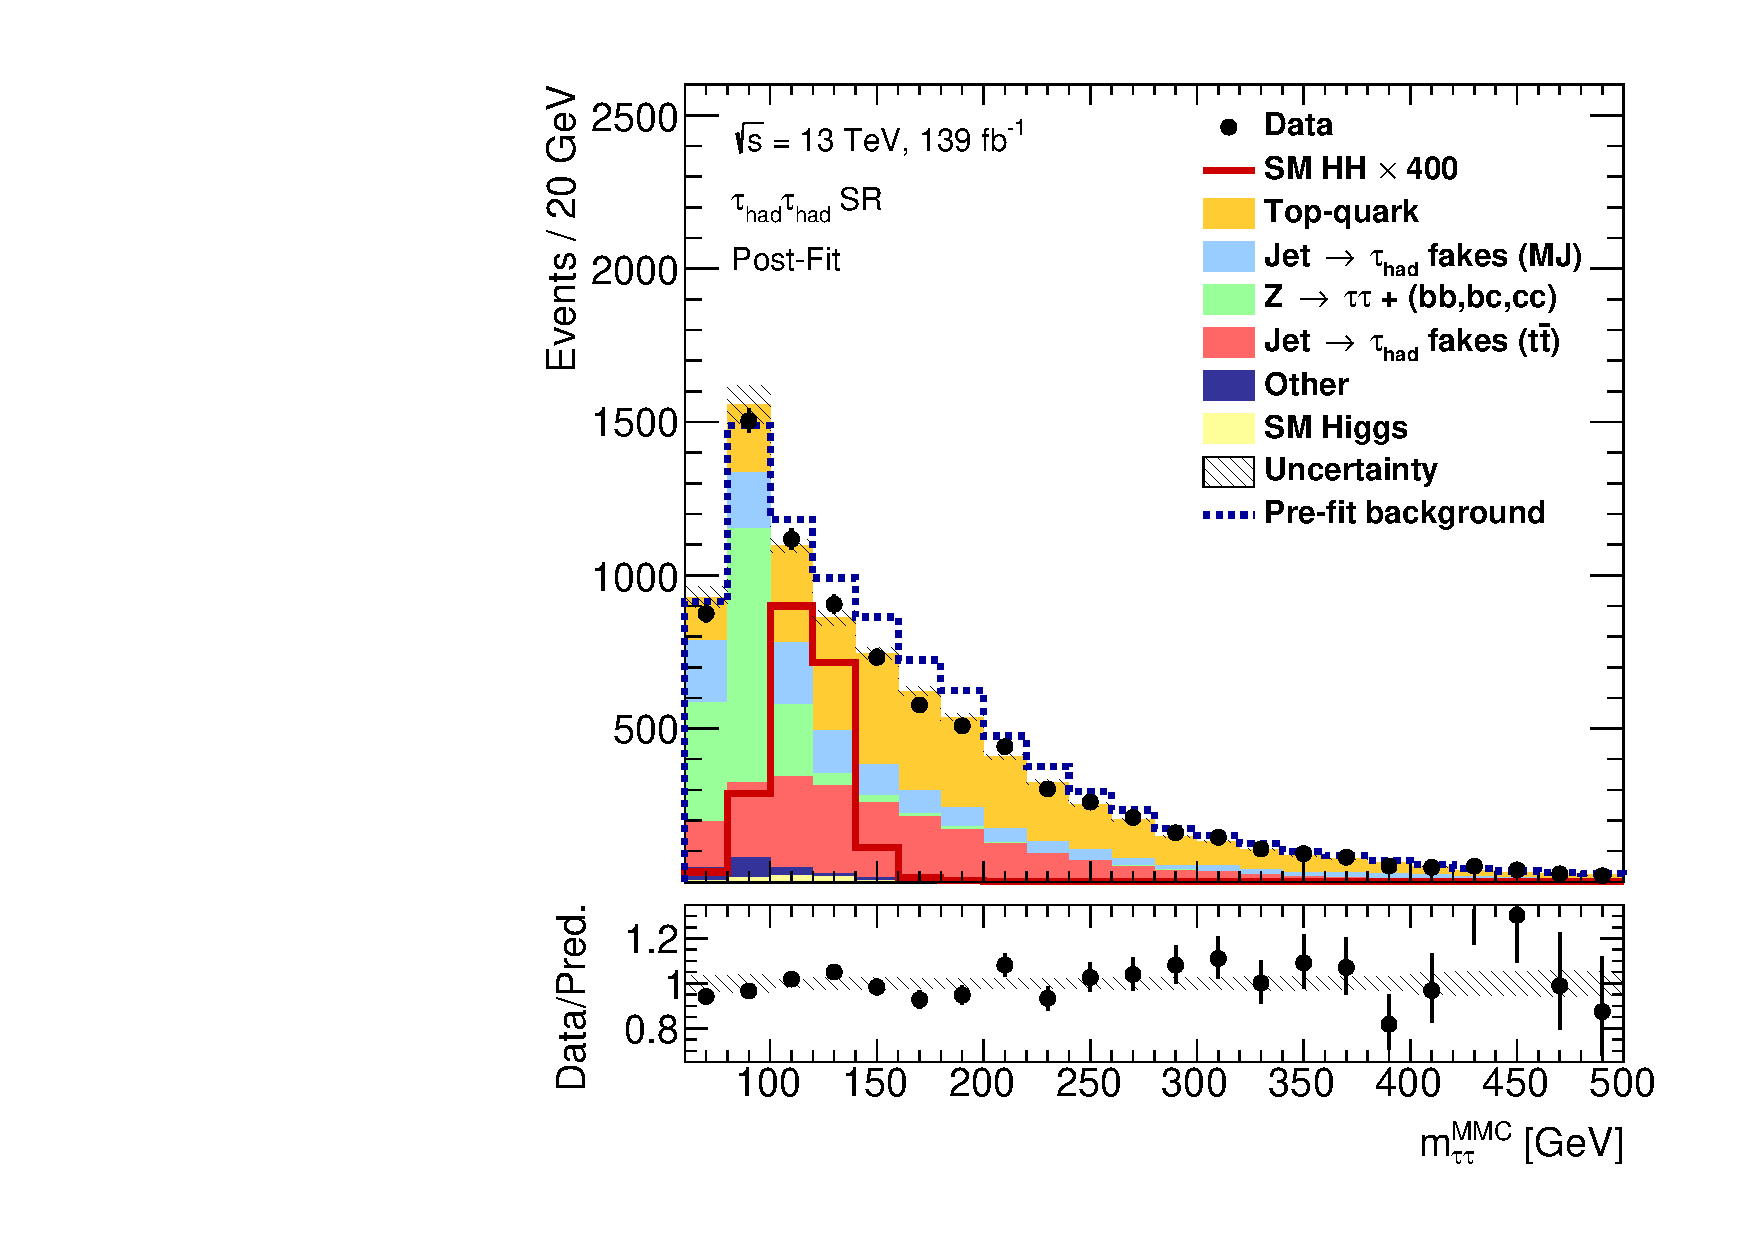
\includegraphics[width=\textwidth]{results_nonres/postfit_mvainputs/Region_BMin0_incJet1_distmMMC_J2_Y2015_DLLOS_T2_SpcTauHH_L0_GlobalFit_conditionnal_mu0}
  \end{subfigure}\hfill%
  \begin{subfigure}{0.46\textwidth}
    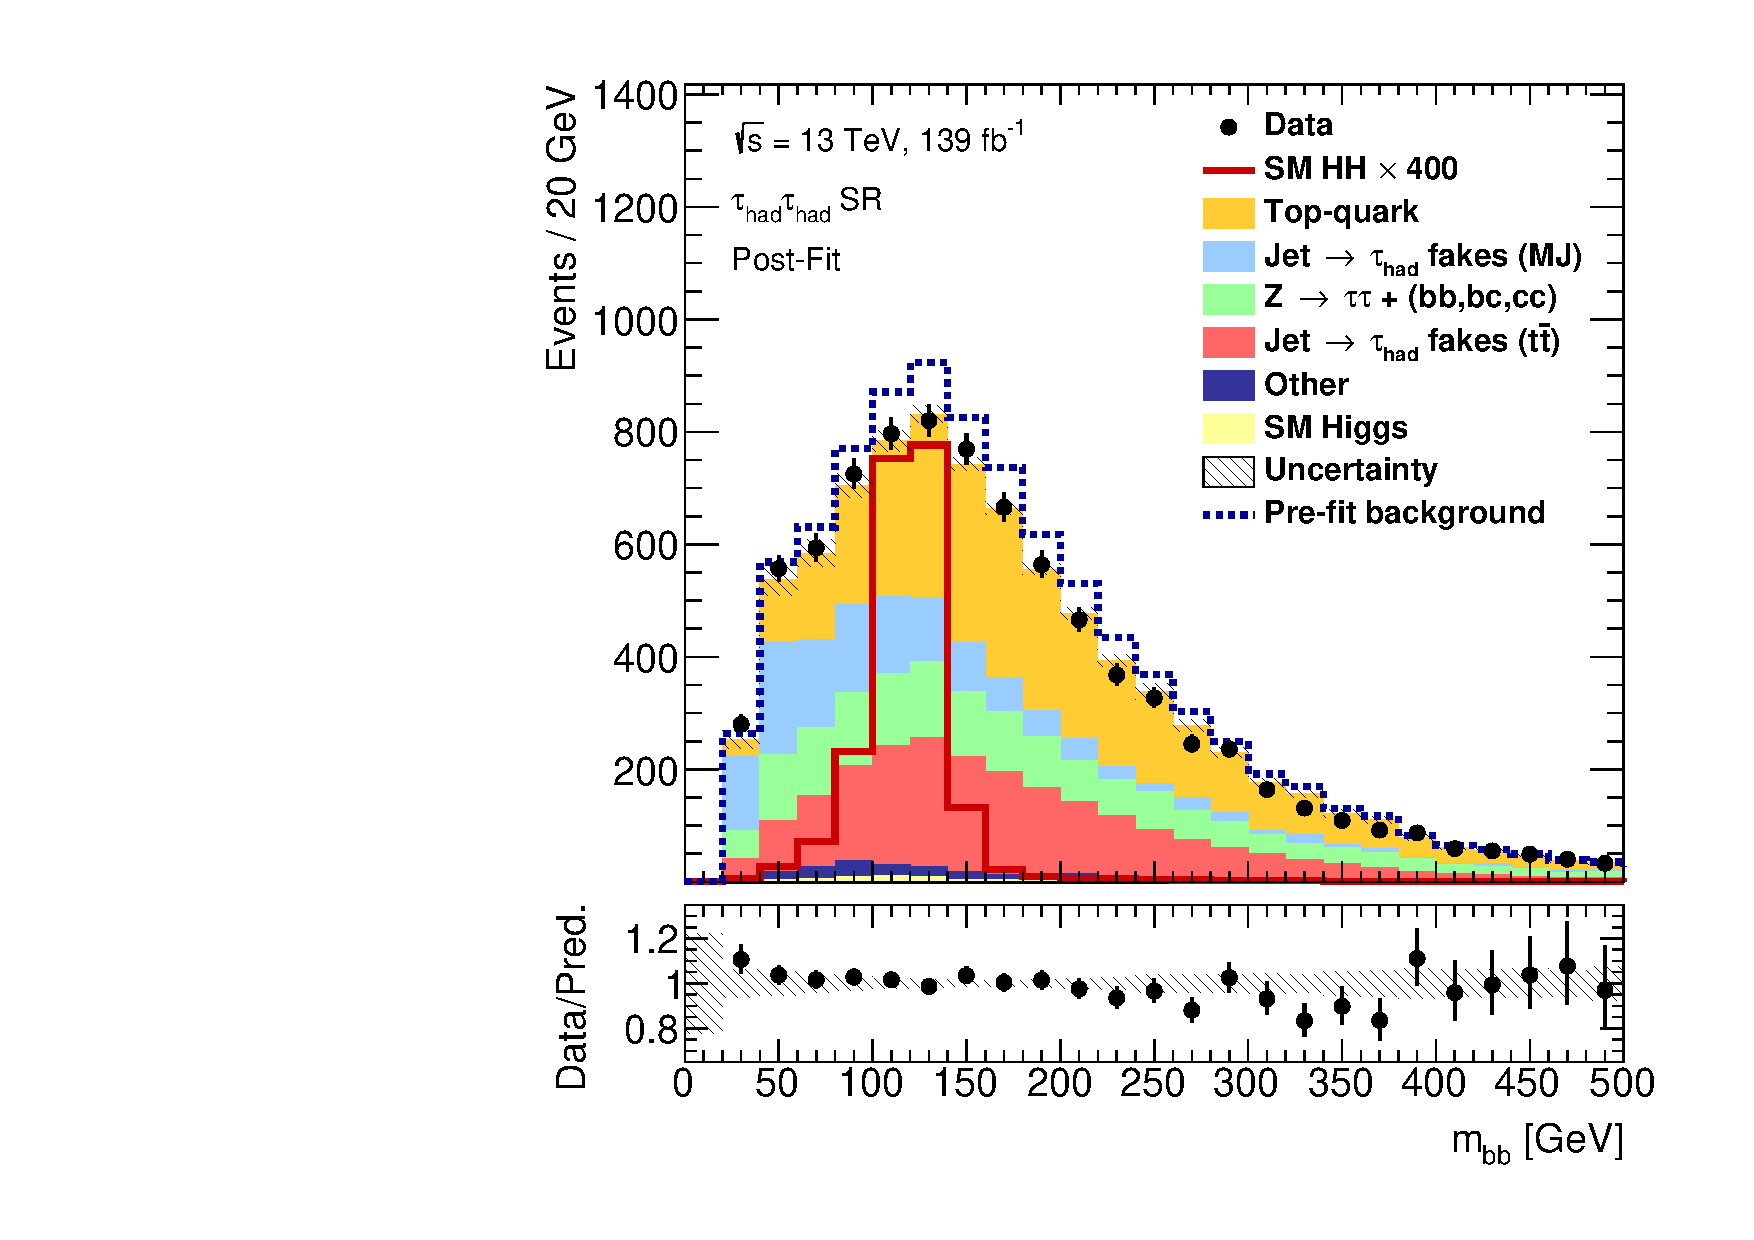
\includegraphics[width=\textwidth]{results_nonres/postfit_mvainputs/Region_BMin0_incJet1_distmBB_J2_Y2015_DLLOS_T2_SpcTauHH_L0_GlobalFit_conditionnal_mu0}
  \end{subfigure}

  \begin{subfigure}{0.46\textwidth}
    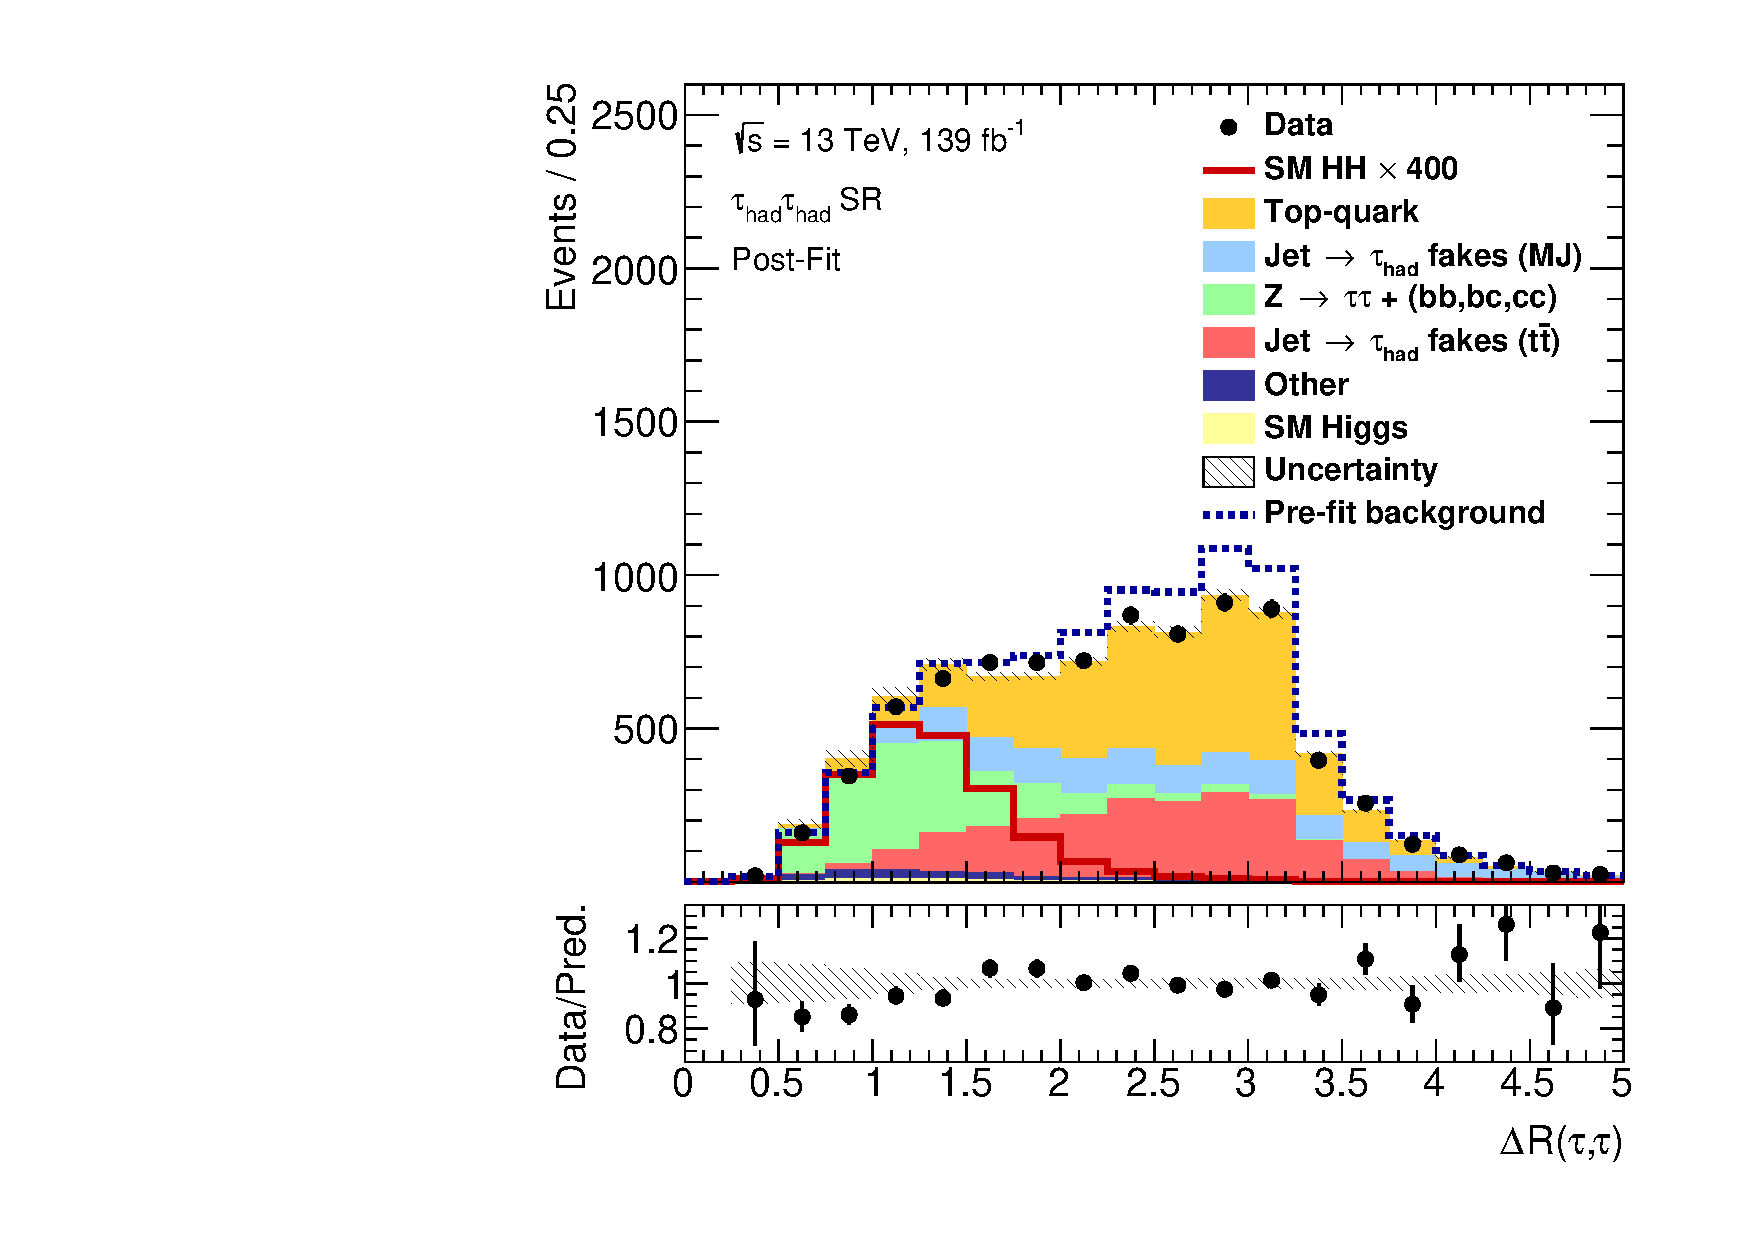
\includegraphics[width=\textwidth]{results_nonres/postfit_mvainputs/Region_BMin0_incJet1_distdRTauTau_J2_Y2015_DLLOS_T2_SpcTauHH_L0_GlobalFit_conditionnal_mu0}
  \end{subfigure}\hfill%
  \begin{subfigure}{0.46\textwidth}
    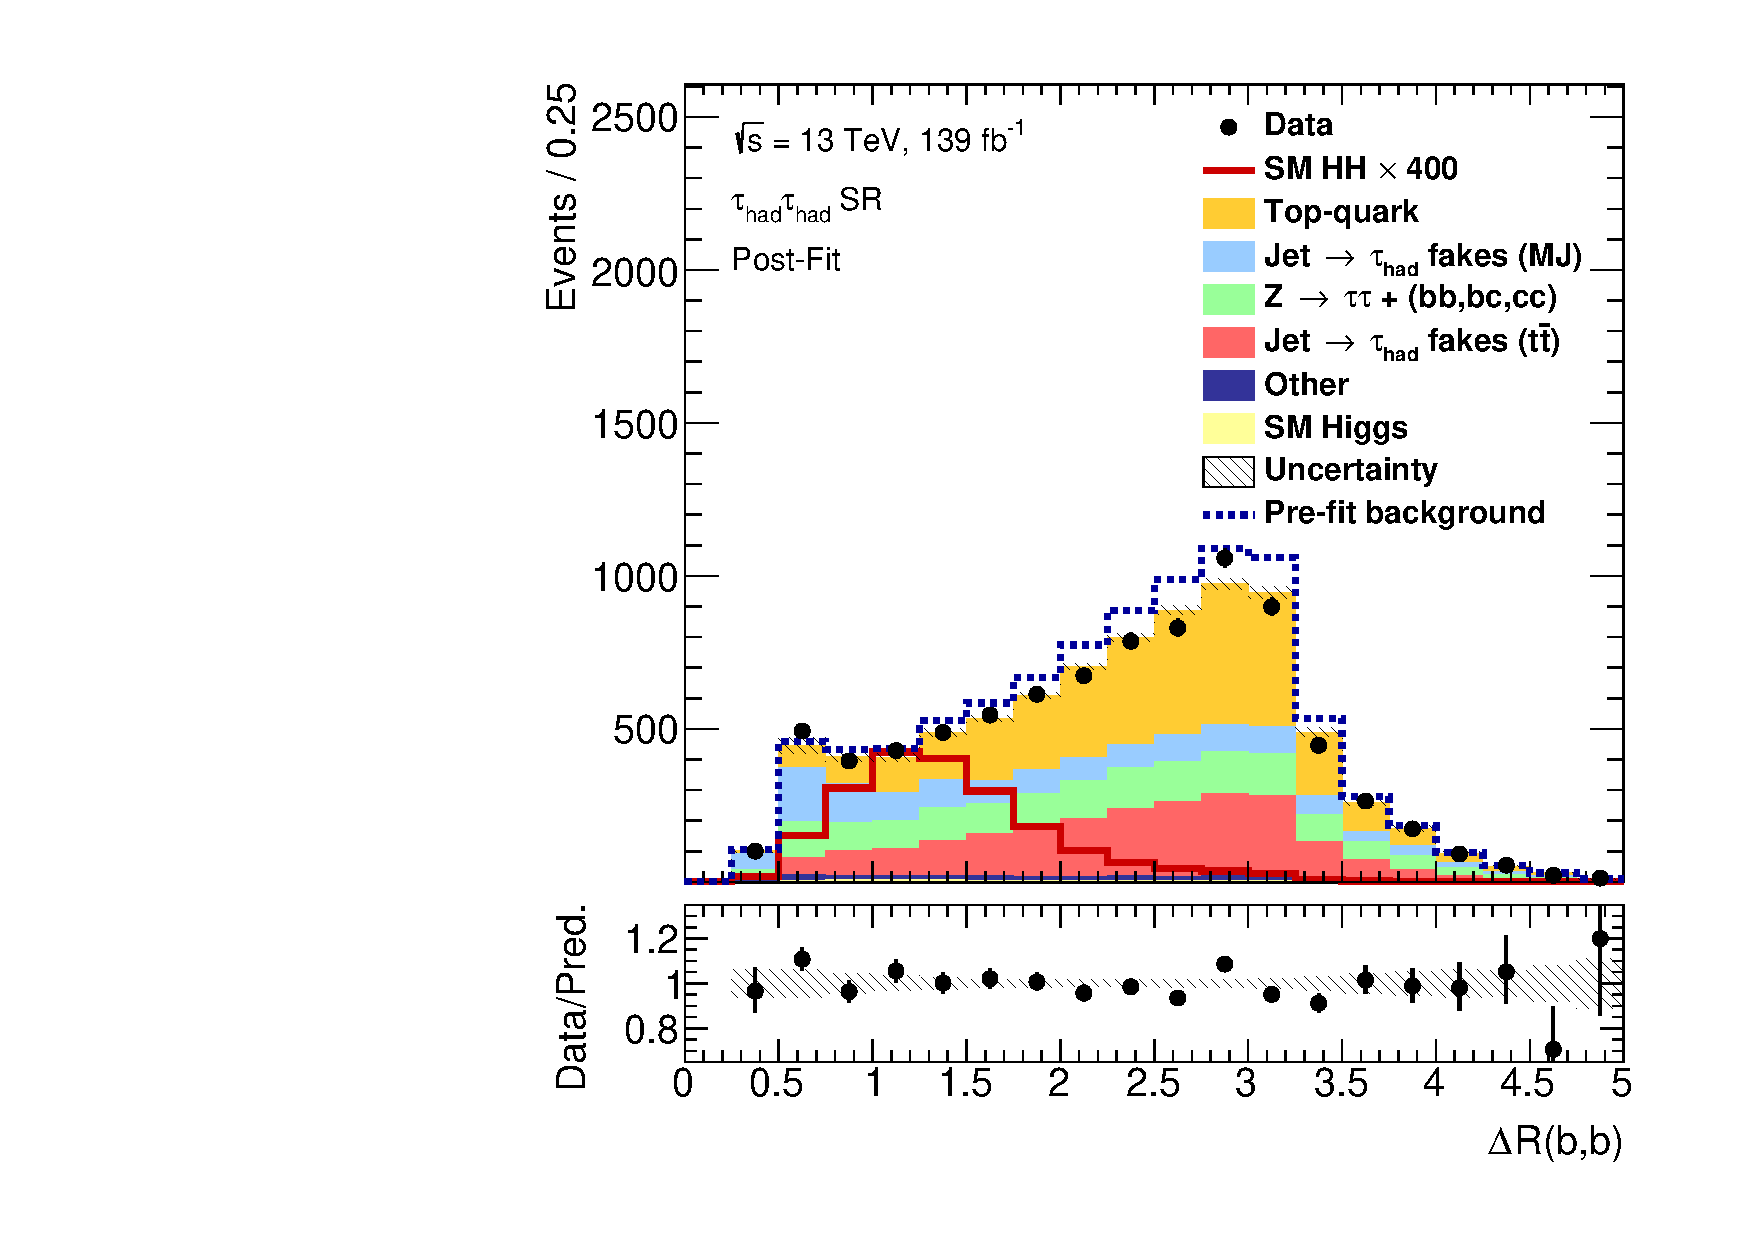
\includegraphics[width=\textwidth]{results_nonres/postfit_mvainputs/Region_BMin0_incJet1_distdRBB_J2_Y2015_DLLOS_T2_SpcTauHH_L0_GlobalFit_conditionnal_mu0}
  \end{subfigure}

  \begin{subfigure}{0.46\textwidth}
    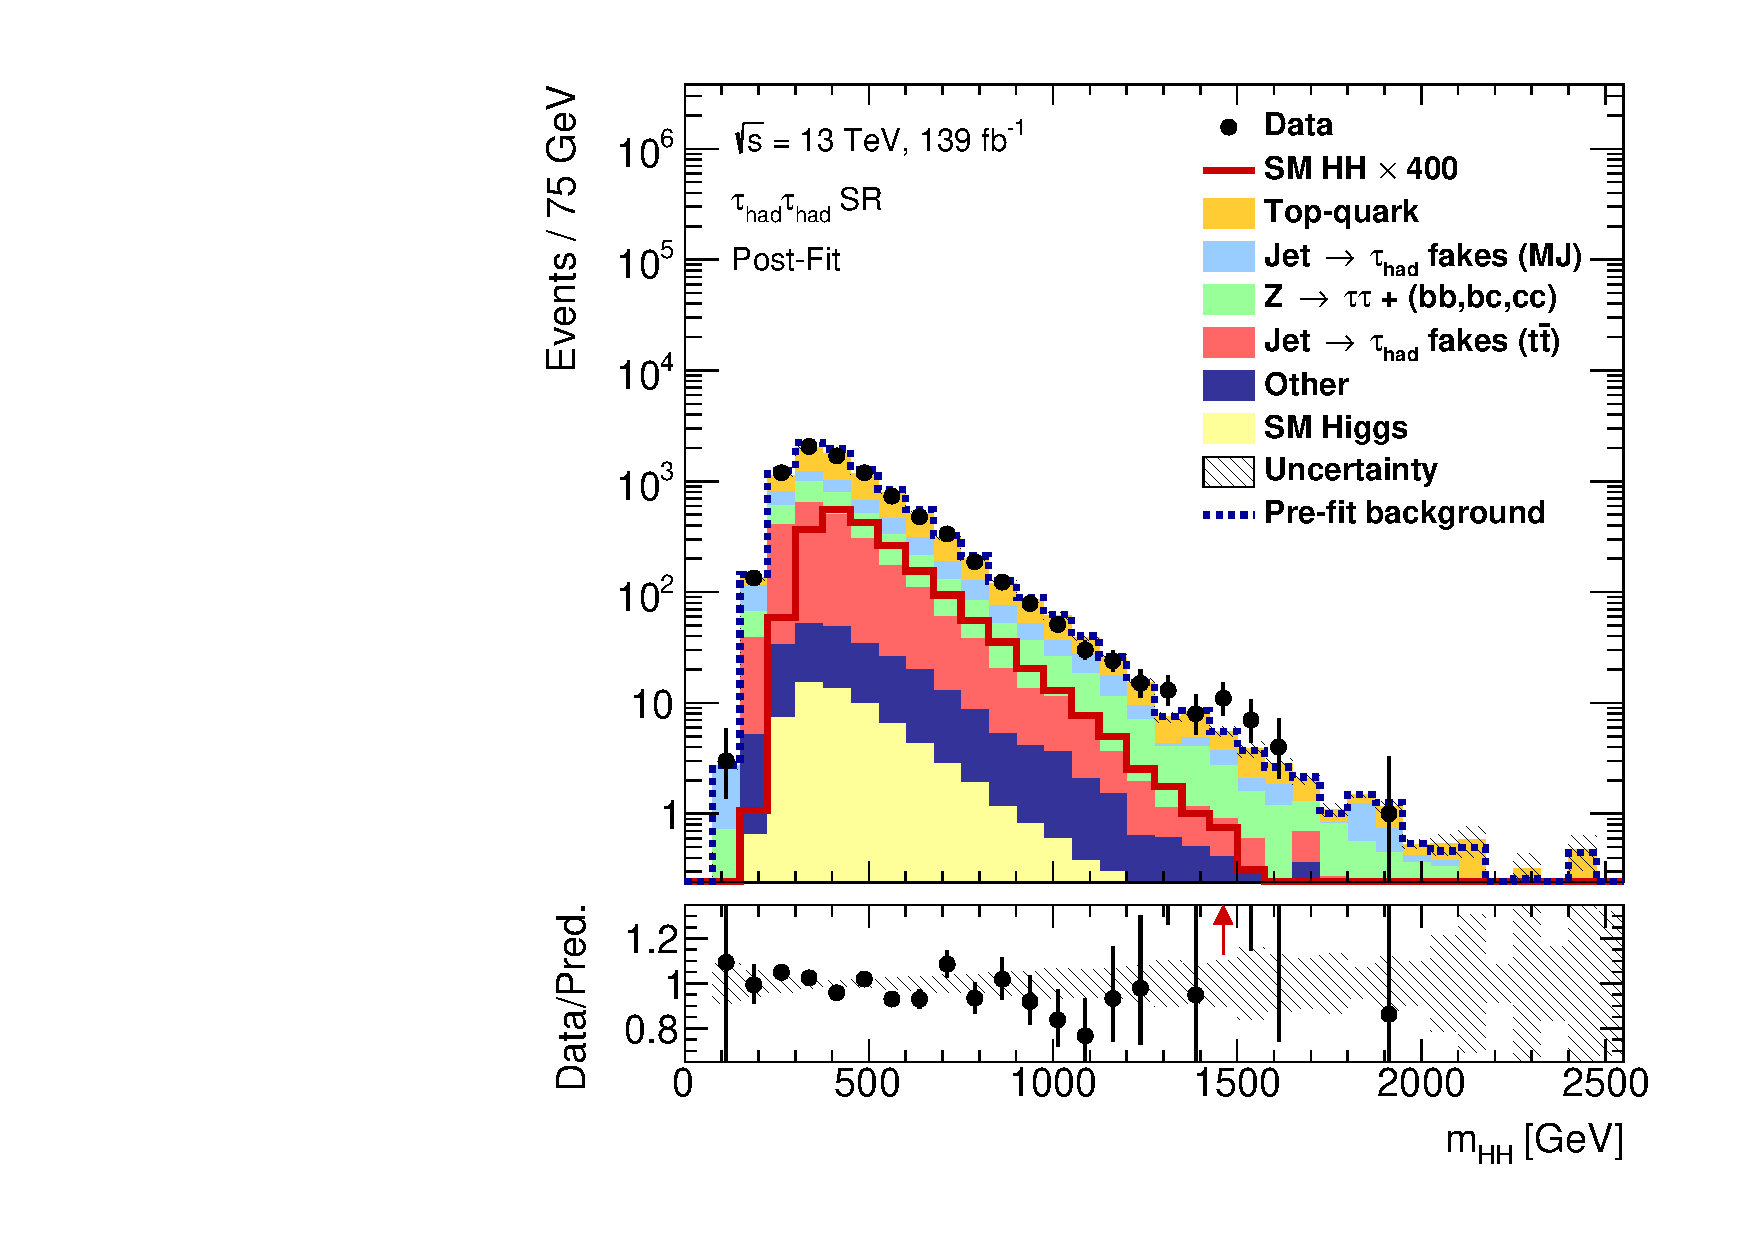
\includegraphics[width=\textwidth]{results_nonres/postfit_mvainputs/Region_BMin0_incJet1_distmHH_J2_Y2015_DLLOS_T2_SpcTauHH_L0_GlobalFit_conditionnal_mu0log}
  \end{subfigure}

  \caption{Distributions of the BDT input variables in the \hadhad
    signal region after the background-only fit of MVA scores and \mll
    in signal and control regions. The expected SM $\HH$ signal is
    overlayed after scaling the normalisation by 400.}
\end{figure}



% q0 (obs): 0.357911
% sig (obs): 0.598257
% pval (obs): 0.274834

% SM (Asimov mu = 1)
% Median significance: 0.667530
% Median pValue: 0.252217

The background-only hypothesis is compared to the alternative of the
background in addition to a positive SM \HH signal with
strength~$\mu$. The likelihood ratio test comparing both hypotheses
yields an observed $p$-value of \SI{27.5}{\percent} (expected
$p$-value of \SI{25.2}{\percent} from the $\mu = 1$ Asimov
dataset). Therefore, the background-only hypothesis cannot be rejected
and thus upper limits on the SM \HH signal strength and cross sections
are placed using the \CLs method.



\todo[inline]{Postfit MVA input plots (hadhad)}
\todo[inline]{Postfit yields: inclusively and in the last (last two) bin(s)?}
\todo[inline]{Postfit norm factors?}

\todo[inline]{Goodness of fit? -> Good fit so set limits.}

\todo[inline]{Postfit ranking: combined, hadhad, lephad}
\todo[inline]{Grouped impact? / Breakdown?}

\begin{table}[htbp]
  \centering

  % Workspaces: comb_2022_01_29
  % ==================
% Channel: combined
% Upper limit on mu:
%         Obs.     -2sigma     -1sigma        Exp.     +1sigma     +2sigma
%     4.700596    2.082483    2.795737    3.879976    5.399804    7.238819

% Upper limit on xsec [fb]:
%         Obs.     -2sigma     -1sigma        Exp.     +1sigma     +2sigma
%     136.6652     61.5679     82.6550    114.7102    159.6434    214.0133

% ==================
% ==================
% Channel: hadhad
% Upper limit on mu:
%         Obs.     -2sigma     -1sigma        Exp.     +1sigma     +2sigma
%     4.951880    2.371052    3.183142    4.417624    6.148054    8.241901

% Upper limit on xsec [fb]:
%         Obs.     -2sigma     -1sigma        Exp.     +1sigma     +2sigma
%     145.1928     70.4159     94.5334    131.1952    182.5858    244.7692

% ==================
% ==================
% Channel: lephad
% Upper limit on mu:
%         Obs.     -2sigma     -1sigma        Exp.     +1sigma     +2sigma
%     9.679448    4.205958    5.646506    7.836325   10.905898   14.620128

% Upper limit on xsec [fb]:
%         Obs.     -2sigma     -1sigma        Exp.     +1sigma     +2sigma
%     281.6663    124.3330    166.9173    231.6509    322.3910    432.1879

% ==================
\begin{tabular}{
  lc
  S[table-format=3.1, round-mode=figures, round-precision=2]
  S[table-format=3.1, round-mode=figures, round-precision=2]
  S[table-format=3.1, round-mode=figures, round-precision=2]
  S[table-format=3.1, round-mode=figures, round-precision=2]
  S[table-format=3.1, round-mode=figures, round-precision=2]
  S[table-format=3.1, round-mode=figures, round-precision=2]
  }
  \toprule
  && {Observed} & {$-2\sigma$} & {$-1\sigma$} & {Expected} & {$+1\sigma$} & {$+2\sigma$} \\
  \midrule
  \multirow{2}{*}{\lephad channel} & {$\xsecggfvbf \, / \, \si{\femto\barn}$} & 281.6663 & 124.3330 & 166.9173 & 231.6509 & 322.3910 & 432.1879 \\
                                   & {$\mu$} & 9.679448 & 4.205958 & 5.646506 & 7.836325 & 10.905898 & 14.620128 \\
  \midrule
  \multirow{2}{*}{\hadhad channel} & {$\xsecggfvbf \, / \, \si{\femto\barn}$} & 145.1928 & 70.4159 & 94.5334 & 131.1952 & 182.5858 & 244.7692 \\
                                   & {$\mu$} & 4.951880 & 2.371052 & 3.183142 & 4.417624 & 6.148054 & 8.241901 \\
  \midrule
  \multirow{2}{*}{Combination}     & {$\xsecggfvbf \, / \, \si{\femto\barn}$} & 136.6652 & 61.5679 & 82.6550 & 114.7102 & 159.6434 & 214.0133 \\
                                   & {$\mu$} & 4.700596 & 2.082483 & 2.795737 & 3.879976 & 5.399804 & 7.238819 \\
  \bottomrule
\end{tabular}

%%% Local Variables:
%%% mode: latex
%%% TeX-master: "../phd_thesis"
%%% End:


  \caption{Upper limits on the total cross section of Higgs pair
    production via ggF and VBF as well as the signal
    strength~$\mu = \sigma_\text{ggF+VBF} /
    \sigma_\text{ggF+VBF}^\text{SM}$ at 95\% $\text{CL}_\text{s}$.}
  \todo[inline]{Make a note somewhere that the cross section upper
    limits are using a different workspace which removes cross section
    uncertainties.}
  \label{tab:limits_non_resonant}
\end{table}


\subsection{Results of the search for resonant production of $HH$}

\todo[inline]{Post fit plots of MVAs}
\todo[inline]{Ranking plots: Selected masses combined only}
\todo[inline]{Pull plots? (+Asimov)}




\begin{figure}[htbp]
  \centering

  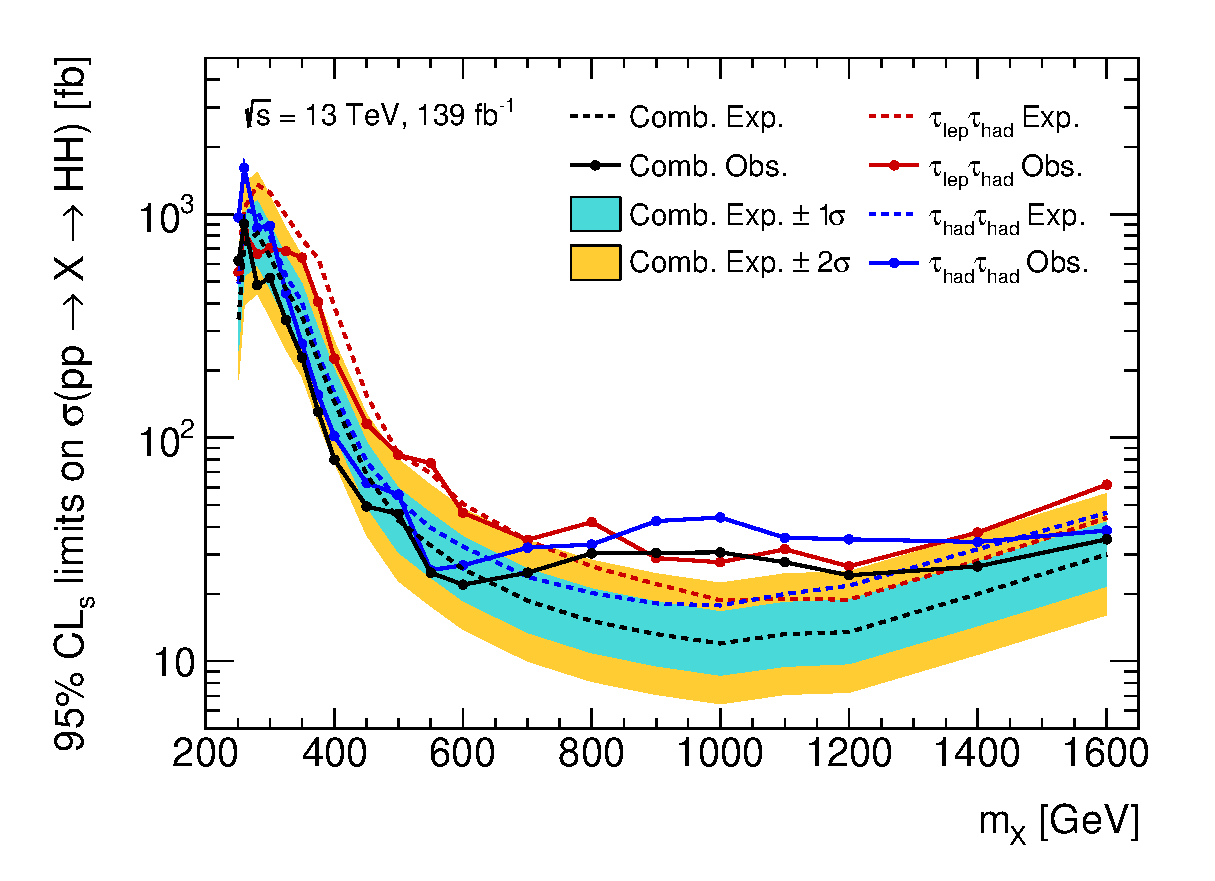
\includegraphics[width=0.65\textwidth]{results/resonant_comb_upper_limits}

  \caption{Upper limits for the resonant search}
  \label{fig:res_upper_limits}
\end{figure}

\begin{figure}[htbp]
  \centering

  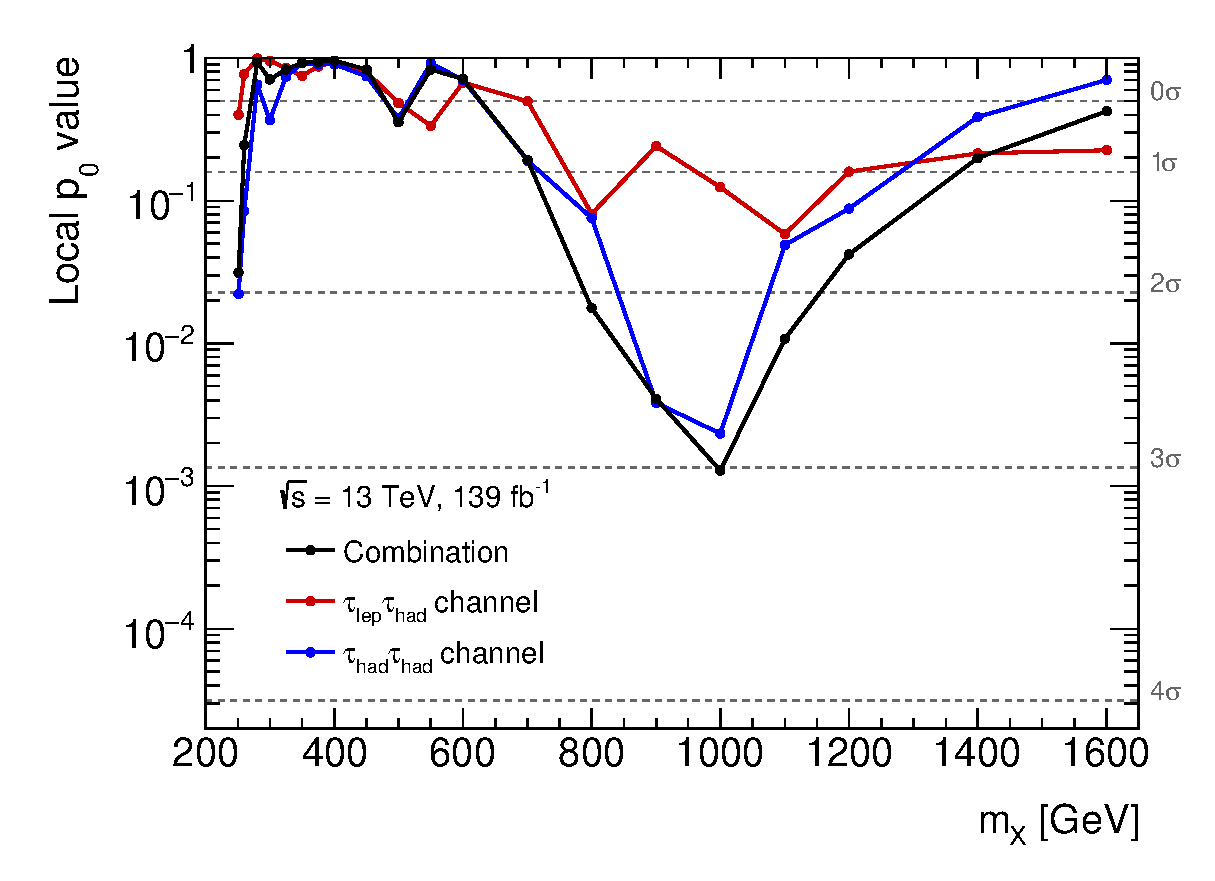
\includegraphics[width=0.65\textwidth]{results/resonant_comb_pvalues}

  \caption{Local pvalue scan}
  \label{fig:local_pvalues}
\end{figure}

\subsection{Global significance estimation of the $\mX = \SI{1000}{\GeV}$ excess}

\subsection{Discussion}

\todo[inline]{What are the limiting factors? Data statistics /
  statistical precision of the bkg estimate (could be improved with a
  better data-driven background estimate).}

\todo[inline]{Systematic uncertainty relatively unimportant at this
  stage.}


\begin{table}[htbp]
  \centering

  \begin{tabular}{lSS}
    \toprule
    & \multicolumn{2}{c}{Expected number of events} \\
    Process & {Last two bins} & {Last bin} \\
    \midrule
    \ZHF & 6.9 & \\
    Single Higgs boson & 6.9 & \\
    \ttbar & 4.6 & \\
    \jettotauhadvis (\ttbar) & 3.4 & \\
    \jettotauhadvis (multi-jet) & 2.2 & \\
    Other & 1.8 & \\
    \midrule
    Total background & & \\
    \midrule
    SM \HH (gluon fusion) & & \\
    SM \HH (VBF) & & \\
    \bottomrule
  \end{tabular}

  \caption{Table of expected yields. The uncertainties are from
    statistical sources only.}
  \todo[inline]{Post-fit yields}
\end{table}


%%% Local Variables:
%%% mode: latex
%%% TeX-master: "../../phd_thesis"
%%% End:
